%%%%%%%%%%%%%%%%%%%%%%%%%%%%%%%%%%%%%%%%%%%%%%%%%%%%%%%%%%%%
% 1.12 LIE GROUPS & LIE ALGEBRAS
% The Composition of Advanced Mathematics
%%%%%%%%%%%%%%%%%%%%%%%%%%%%%%%%%%%%%%%%%%%%%%%%%%%%%%%%%%%%

\section{Lie Groups and Lie Algebras}
\label{sec:lie-groups-lie-algebras}

\prerequisite{
Linear algebra from \cref{sec:linear-algebra}, group theory from
\cref{sec:group-theory}, field theory from \cref{sec:field-theory}, and
representation theory from \cref{sec:representation-theory}. Familiarity with
multivariable calculus and differential geometry is helpful for the geometric
parts of this section, but the principal algebraic constructions are developed
here directly.
}

\learningobjectives{
By the end of this section, the reader should be able to:
\begin{itemize}
    \item explain why Lie groups combine continuous geometry with group structure;
    \item recognize important matrix Lie groups such as \(GL_n\), \(SL_n\), \(O(n)\), \(SO(n)\), and \(U(n)\);
    \item identify the tangent space at the identity of a Lie group;
    \item define a Lie algebra and the Lie bracket;
    \item verify the alternating and Jacobi identities;
    \item compute matrix commutators;
    \item distinguish abelian and nonabelian Lie algebras;
    \item recognize the classical matrix Lie algebras \(\mathfrak{gl}_n\), \(\mathfrak{sl}_n\), \(\mathfrak{so}_n\), and \(\mathfrak{u}_n\);
    \item explain the relationship between one-parameter subgroups and the exponential map;
    \item compute basic matrix exponentials;
    \item define Lie subalgebras, ideals, centers, and homomorphisms;
    \item understand the adjoint representation;
    \item recognize structure constants and basic examples of Lie algebra representations;
    \item explain how local Lie algebra information reflects the structure of a Lie group;
    \item connect Lie theory with geometry, differential equations, symmetry, and mathematical physics.
\end{itemize}
}

%%%%%%%%%%%%%%%%%%%%%%%%%%%%%%%%%%%%%%%%%%%%%%%%%%%%%%%%%%%%
\subsection{Continuous Symmetry}
\label{subsec:continuous-symmetry}
%%%%%%%%%%%%%%%%%%%%%%%%%%%%%%%%%%%%%%%%%%%%%%%%%%%%%%%%%%%%

Many groups encountered earlier are discrete.

For example,

\[ S_n,\qquad C_n,\qquad D_n \]

contain individual group elements separated from one another.

Other symmetry groups vary continuously.

A rotation of the plane can occur through any real angle

\[ \theta\in\R. \]

As \(\theta\) changes continuously, the corresponding rotation matrix

\[ R(\theta)=
\begin{pmatrix}
\cos\theta&-\sin\theta\\
\sin\theta&\cos\theta
\end{pmatrix} \]

also changes continuously.

This produces a group that is simultaneously an algebraic object and a
geometric space.

\begin{conceptbox}
Lie theory studies continuous symmetry.

A Lie group combines a group structure with a smooth geometric structure,
while a Lie algebra describes the group's infinitesimal behavior near its
identity.
\end{conceptbox}

%%%%%%%%%%%%%%%%%%%%%%%%%%%%%%%%%%%%%%%%%%%%%%%%%%%%%%%%%%%%
\subsection{From Discrete to Continuous Symmetry}
\label{subsec:discrete-continuous-symmetry}
%%%%%%%%%%%%%%%%%%%%%%%%%%%%%%%%%%%%%%%%%%%%%%%%%%%%%%%%%%%%

The distinction can be visualized schematically.

\begin{center}
\begin{tikzpicture}[
    node distance=17mm,
    box/.style={draw,rounded corners,align=center,inner sep=6pt},
    >=stealth
]
\node[box] (disc) {Discrete symmetry\\\(C_n,D_n,S_n\)};
\node[box,right=of disc] (cont) {Continuous symmetry\\rotations, translations};
\node[box,right=of cont] (lie) {Lie groups};
\node[box,below=of lie] (alg) {Lie algebras\\infinitesimal symmetry};

\draw[->,thick] (disc)--node[above]{generalize}(cont);
\draw[->,thick] (cont)--(lie);
\draw[->,thick] (lie)--node[right]{differentiate}(alg);
\end{tikzpicture}
\end{center}

%%%%%%%%%%%%%%%%%%%%%%%%%%%%%%%%%%%%%%%%%%%%%%%%%%%%%%%%%%%%
\subsection{What Is a Lie Group?}
\label{subsec:lie-group-definition}
%%%%%%%%%%%%%%%%%%%%%%%%%%%%%%%%%%%%%%%%%%%%%%%%%%%%%%%%%%%%

A precise definition uses the language of smooth manifolds, whose canonical
development belongs to geometry and topology.

For the present algebraic treatment, the essential idea is the following.

\begin{definitionbox}{Lie Group}
A \emph{Lie group} is a group \(G\) that is also a smooth manifold such that
the multiplication map
\[ (g,h)\longmapsto gh \]
and inversion map
\[ g\longmapsto g^{-1} \]
are smooth.
\end{definitionbox}

Thus algebraic multiplication and geometric smoothness are compatible.

%%%%%%%%%%%%%%%%%%%%%%%%%%%%%%%%%%%%%%%%%%%%%%%%%%%%%%%%%%%%
\subsection{The Real Numbers as a Lie Group}
\label{subsec:real-line-lie-group}
%%%%%%%%%%%%%%%%%%%%%%%%%%%%%%%%%%%%%%%%%%%%%%%%%%%%%%%%%%%%

The additive group

\[ (\R,+) \]

is one of the simplest Lie groups.

Its identity is

\[ 0, \]

its inverse operation is

\[ x\mapsto -x, \]

and multiplication in the group means ordinary addition:

\[ (x,y)\mapsto x+y. \]

Both operations vary smoothly with the real variables.

%%%%%%%%%%%%%%%%%%%%%%%%%%%%%%%%%%%%%%%%%%%%%%%%%%%%%%%%%%%%
\subsection{The Multiplicative Positive Reals}
\label{subsec:positive-reals-lie-group}
%%%%%%%%%%%%%%%%%%%%%%%%%%%%%%%%%%%%%%%%%%%%%%%%%%%%%%%%%%%%

The set

\[ \R_{>0}=\{x\in\R:x>0\} \]

forms a Lie group under multiplication.

The exponential function connects it to the additive real numbers:

\[ \exp:\R\to\R_{>0},\qquad x\mapsto e^x. \]

Because

\[ e^{x+y}=e^xe^y, \]

the exponential function is a group homomorphism.

In fact,

\[ (\R,+)\cong(\R_{>0},\cdot). \]

%%%%%%%%%%%%%%%%%%%%%%%%%%%%%%%%%%%%%%%%%%%%%%%%%%%%%%%%%%%%
\subsection{The Circle Group}
\label{subsec:circle-group}
%%%%%%%%%%%%%%%%%%%%%%%%%%%%%%%%%%%%%%%%%%%%%%%%%%%%%%%%%%%%

Consider

\[ S^1=\{z\in\C:|z|=1\}. \]

The notation \(S^1\) is read ``\(S\) one'' and denotes the unit circle.

Every element can be written

\[ z=e^{i\theta}. \]

Multiplication gives

\[ e^{i\theta}e^{i\phi}=e^{i(\theta+\phi)}. \]

Thus angle addition corresponds to group multiplication.

\begin{center}
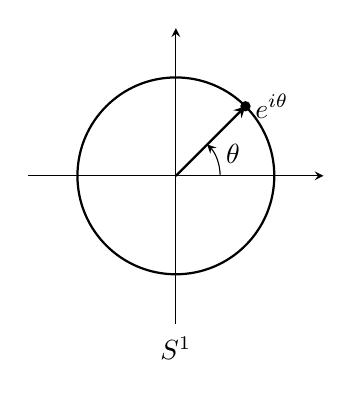
\begin{tikzpicture}[scale=1.25,>=stealth]
\draw[->] (-1.5,0)--(1.5,0);
\draw[->] (0,-1.5)--(0,1.5);
\draw[thick] (0,0) circle (1);

\coordinate (P) at ({cos(45)},{sin(45)});
\fill (P) circle (1.5pt);
\draw[->,thick] (0,0)--(P);
\draw[->] (0.45,0) arc[start angle=0,end angle=45,radius=0.45];

\node at (0.58,0.22) {\(\theta\)};
\node[right] at (P) {\(e^{i\theta}\)};
\node at (0,-1.75) {\(S^1\)};
\end{tikzpicture}
\end{center}

%%%%%%%%%%%%%%%%%%%%%%%%%%%%%%%%%%%%%%%%%%%%%%%%%%%%%%%%%%%%
\subsection{Matrix Lie Groups}
\label{subsec:matrix-lie-groups}
%%%%%%%%%%%%%%%%%%%%%%%%%%%%%%%%%%%%%%%%%%%%%%%%%%%%%%%%%%%%

Many of the most important Lie groups consist of matrices.

These are called \emph{matrix Lie groups}.

The central example is the general linear group

\[ GL_n(\R)=\{A\in M_n(\R):\det(A)\neq0\}. \]

The notation

\[ GL_n(\R) \]

is read ``general linear group of degree \(n\) over the real numbers.''

Its operation is matrix multiplication.

%%%%%%%%%%%%%%%%%%%%%%%%%%%%%%%%%%%%%%%%%%%%%%%%%%%%%%%%%%%%
\subsection{The General Linear Group}
\label{subsec:general-linear-lie-group}
%%%%%%%%%%%%%%%%%%%%%%%%%%%%%%%%%%%%%%%%%%%%%%%%%%%%%%%%%%%%

Because matrix multiplication and matrix inversion vary smoothly wherever the
determinant is nonzero,

\[ GL_n(\R) \]

is a Lie group.

Likewise,

\[ GL_n(\C) \]

is a complex matrix Lie group.

Its elements represent all invertible linear transformations of
\(\R^n\) or \(\C^n\).

%%%%%%%%%%%%%%%%%%%%%%%%%%%%%%%%%%%%%%%%%%%%%%%%%%%%%%%%%%%%
\subsection{The Special Linear Group}
\label{subsec:special-linear-group}
%%%%%%%%%%%%%%%%%%%%%%%%%%%%%%%%%%%%%%%%%%%%%%%%%%%%%%%%%%%%

\begin{definitionbox}{Special Linear Group}
The \emph{special linear group} is
\[ SL_n(F)=\{A\in GL_n(F):\det(A)=1\}. \]
\end{definitionbox}

The notation

\[ SL_n(F) \]

is read ``special linear group of degree \(n\) over \(F\).''

The word \emph{special} refers to the determinant-one condition.

Since

\[ \det(AB)=\det(A)\det(B), \]

the product of two determinant-one matrices again has determinant one.

%%%%%%%%%%%%%%%%%%%%%%%%%%%%%%%%%%%%%%%%%%%%%%%%%%%%%%%%%%%%
\subsection{Orthogonal Groups}
\label{subsec:orthogonal-groups}
%%%%%%%%%%%%%%%%%%%%%%%%%%%%%%%%%%%%%%%%%%%%%%%%%%%%%%%%%%%%

\begin{definitionbox}{Orthogonal Group}
The \emph{orthogonal group} is
\[ O(n)=\{A\in GL_n(\R):A^{\mathsf T}A=I\}. \]
\end{definitionbox}

Orthogonal matrices preserve the Euclidean inner product:

\[ \inner{Av,Aw}=\inner{v,w}. \]

Consequently, they preserve lengths and angles.

The group \(O(n)\) contains rotations and reflections of \(\R^n\).

%%%%%%%%%%%%%%%%%%%%%%%%%%%%%%%%%%%%%%%%%%%%%%%%%%%%%%%%%%%%
\subsection{The Special Orthogonal Group}
\label{subsec:special-orthogonal-group}
%%%%%%%%%%%%%%%%%%%%%%%%%%%%%%%%%%%%%%%%%%%%%%%%%%%%%%%%%%%%

\begin{definitionbox}{Special Orthogonal Group}
The \emph{special orthogonal group} is
\[ SO(n)=\{A\in O(n):\det(A)=1\}. \]
\end{definitionbox}

The notation

\[ SO(n) \]

is read ``special orthogonal group of degree \(n\).''

Elements of \(SO(n)\) represent orientation-preserving orthogonal
transformations.

In particular,

\[ SO(2) \]

is the group of rotations of the plane.

%%%%%%%%%%%%%%%%%%%%%%%%%%%%%%%%%%%%%%%%%%%%%%%%%%%%%%%%%%%%
\subsection{The Group \(SO(2)\)}
\label{subsec:so2}
%%%%%%%%%%%%%%%%%%%%%%%%%%%%%%%%%%%%%%%%%%%%%%%%%%%%%%%%%%%%

Every element of \(SO(2)\) has the form

\[ R(\theta)=
\begin{pmatrix}
\cos\theta&-\sin\theta\\
\sin\theta&\cos\theta
\end{pmatrix}. \]

Matrix multiplication gives

\[ R(\theta)R(\phi)=R(\theta+\phi). \]

Thus

\[ SO(2)\cong S^1. \]

\begin{center}
\begin{tikzpicture}[scale=1.05,>=stealth]
\draw[->] (-2.1,0)--(2.1,0);
\draw[->] (0,-2.1)--(0,2.1);
\draw[thick,->] (0,0)--(1.55,0) node[right]{\(v\)};
\draw[thick,->] (0,0)--({1.55*cos(70)},{1.55*sin(70)})
node[above]{\(R(\theta)v\)};
\draw[->] (0.65,0) arc[start angle=0,end angle=70,radius=0.65];
\node at (0.78,0.43) {\(\theta\)};
\end{tikzpicture}
\end{center}

%%%%%%%%%%%%%%%%%%%%%%%%%%%%%%%%%%%%%%%%%%%%%%%%%%%%%%%%%%%%
\subsection{Unitary Groups}
\label{subsec:unitary-groups}
%%%%%%%%%%%%%%%%%%%%%%%%%%%%%%%%%%%%%%%%%%%%%%%%%%%%%%%%%%%%

For a complex matrix \(A\), let

\[ A^*=\overline{A}^{\mathsf T} \]

denote its conjugate transpose.

\begin{definitionbox}{Unitary Group}
The \emph{unitary group} is
\[ U(n)=\{A\in GL_n(\C):A^*A=I\}. \]
\end{definitionbox}

Unitary transformations preserve the complex inner product.

The subgroup

\[ SU(n)=\{A\in U(n):\det(A)=1\} \]

is called the \emph{special unitary group}.

These groups are fundamental in mathematical physics.

%%%%%%%%%%%%%%%%%%%%%%%%%%%%%%%%%%%%%%%%%%%%%%%%%%%%%%%%%%%%
\subsection{Important Matrix Lie Groups}
\label{subsec:important-matrix-lie-groups}
%%%%%%%%%%%%%%%%%%%%%%%%%%%%%%%%%%%%%%%%%%%%%%%%%%%%%%%%%%%%

\begin{center}
\begin{tabularx}{0.96\textwidth}{@{}lXX@{}}
\toprule
\textbf{Group} & \textbf{Defining condition} & \textbf{Interpretation}\\
\midrule
\(GL_n(\R)\) & \(\det A\neq0\) & invertible real transformations\\
\(SL_n(\R)\) & \(\det A=1\) & volume-preserving linear transformations\\
\(O(n)\) & \(A^{\mathsf T}A=I\) & length-preserving transformations\\
\(SO(n)\) & \(A^{\mathsf T}A=I,\ \det A=1\) & rotations and related orientation-preserving symmetries\\
\(U(n)\) & \(A^*A=I\) & complex inner-product-preserving transformations\\
\(SU(n)\) & \(A^*A=I,\ \det A=1\) & special unitary transformations\\
\bottomrule
\end{tabularx}
\end{center}

%%%%%%%%%%%%%%%%%%%%%%%%%%%%%%%%%%%%%%%%%%%%%%%%%%%%%%%%%%%%
\subsection{Infinitesimal Symmetry}
\label{subsec:infinitesimal-symmetry}
%%%%%%%%%%%%%%%%%%%%%%%%%%%%%%%%%%%%%%%%%%%%%%%%%%%%%%%%%%%%

A Lie group may be complicated globally.

Near its identity, however, it behaves approximately like a vector space.

The tangent space at the identity captures these infinitesimal directions.

If \(G\) is a Lie group with identity \(e\), denote this tangent space by

\[ T_eG. \]

The notation is read:

``the tangent space of \(G\) at the identity \(e\).''

This vector space becomes a Lie algebra.

\begin{center}
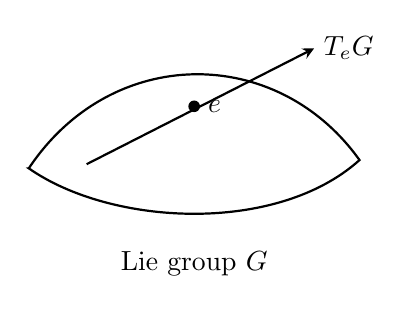
\begin{tikzpicture}[scale=1.05,>=stealth]
\draw[thick] (-2,-0.3)
    .. controls (-1,1.2) and (1,1.2) .. (2,-0.2)
    .. controls (1,-1.1) and (-1,-1.0) .. cycle;

\fill (0,0.45) circle (2pt);
\node[right] at (0.05,0.45) {\(e\)};

\draw[->,thick] (-1.3,-0.25)--(1.45,1.15);
\node[right] at (1.45,1.15) {\(T_eG\)};

\node at (0,-1.45) {Lie group \(G\)};
\end{tikzpicture}
\end{center}

%%%%%%%%%%%%%%%%%%%%%%%%%%%%%%%%%%%%%%%%%%%%%%%%%%%%%%%%%%%%
\subsection{What Is a Lie Algebra?}
\label{subsec:lie-algebra-definition}
%%%%%%%%%%%%%%%%%%%%%%%%%%%%%%%%%%%%%%%%%%%%%%%%%%%%%%%%%%%%

Lie algebras abstract the infinitesimal structure found in Lie groups.

\begin{definitionbox}{Lie Algebra}
A \emph{Lie algebra} over a field \(F\) is a vector space \(\mathfrak g\)
together with a bilinear operation
\[ [\,\cdot,\cdot\,]:\mathfrak g\times\mathfrak g\to\mathfrak g \]
called the \emph{Lie bracket}, satisfying
\[ [X,X]=0 \]
and
\[ [X,[Y,Z]]+[Y,[Z,X]]+[Z,[X,Y]]=0 \]
for all \(X,Y,Z\in\mathfrak g\).
\end{definitionbox}

The second identity is called the \emph{Jacobi identity}.

The notation

\[ [X,Y] \]

is read ``the Lie bracket of \(X\) and \(Y\).''

%%%%%%%%%%%%%%%%%%%%%%%%%%%%%%%%%%%%%%%%%%%%%%%%%%%%%%%%%%%%
\subsection{The Lie Bracket}
\label{subsec:lie-bracket}
%%%%%%%%%%%%%%%%%%%%%%%%%%%%%%%%%%%%%%%%%%%%%%%%%%%%%%%%%%%%

The Lie bracket is bilinear:

\[ [aX+bY,Z]=a[X,Z]+b[Y,Z], \]

and

\[ [X,aY+bZ]=a[X,Y]+b[X,Z]. \]

The condition

\[ [X,X]=0 \]

is called \emph{alternation}.

Over fields of characteristic not equal to \(2\), alternation implies

\[ [X,Y]=-[Y,X]. \]

This property is called \emph{antisymmetry} or \emph{skew-symmetry}.

%%%%%%%%%%%%%%%%%%%%%%%%%%%%%%%%%%%%%%%%%%%%%%%%%%%%%%%%%%%%
\subsection{The Jacobi Identity}
\label{subsec:jacobi-identity}
%%%%%%%%%%%%%%%%%%%%%%%%%%%%%%%%%%%%%%%%%%%%%%%%%%%%%%%%%%%%

The Jacobi identity is

\[ [X,[Y,Z]]+[Y,[Z,X]]+[Z,[X,Y]]=0. \]

It replaces associativity as the central structural identity of a Lie
algebra.

\begin{importantbox}
A Lie bracket is generally \emph{not} associative.

One should not expect
\[ [X,[Y,Z]]=[[X,Y],Z]. \]

Instead, the bracket satisfies the Jacobi identity.
\end{importantbox}

%%%%%%%%%%%%%%%%%%%%%%%%%%%%%%%%%%%%%%%%%%%%%%%%%%%%%%%%%%%%
\subsection{Matrix Commutators}
\label{subsec:matrix-commutators}
%%%%%%%%%%%%%%%%%%%%%%%%%%%%%%%%%%%%%%%%%%%%%%%%%%%%%%%%%%%%

The most important example of a Lie bracket comes from matrices.

For matrices \(X\) and \(Y\), define

\[ [X,Y]=XY-YX. \]

\begin{definitionbox}{Commutator}
The expression
\[ [X,Y]=XY-YX \]
is called the \emph{commutator} of \(X\) and \(Y\).
\end{definitionbox}

The commutator measures failure of multiplication to commute.

Indeed,

\[ [X,Y]=0\iff XY=YX. \]

%%%%%%%%%%%%%%%%%%%%%%%%%%%%%%%%%%%%%%%%%%%%%%%%%%%%%%%%%%%%
\subsection{Worked Example: Matrix Commutator}
\label{subsec:worked-matrix-commutator}
%%%%%%%%%%%%%%%%%%%%%%%%%%%%%%%%%%%%%%%%%%%%%%%%%%%%%%%%%%%%

\begin{workedexamplebox}{Computing a Lie Bracket}

Let

\[ X=\begin{pmatrix}0&1\\0&0\end{pmatrix},\qquad
Y=\begin{pmatrix}0&0\\1&0\end{pmatrix}. \]

Compute \([X,Y]\).

\begin{tabularx}{\textwidth}{@{}>{\raggedright\arraybackslash}p{0.42\textwidth}X@{}}
Compute \(XY\). &
\(\displaystyle XY=\begin{pmatrix}1&0\\0&0\end{pmatrix}\)\\
Compute \(YX\). &
\(\displaystyle YX=\begin{pmatrix}0&0\\0&1\end{pmatrix}\)\\
Subtract. &
\(\displaystyle [X,Y]=XY-YX=\begin{pmatrix}1&0\\0&-1\end{pmatrix}\)
\end{tabularx}

\begin{answerbox}
\[ \boxed{[X,Y]=\begin{pmatrix}1&0\\0&-1\end{pmatrix}} \]
\end{answerbox}
\end{workedexamplebox}

%%%%%%%%%%%%%%%%%%%%%%%%%%%%%%%%%%%%%%%%%%%%%%%%%%%%%%%%%%%%
\subsection{Why the Commutator Is a Lie Bracket}
\label{subsec:commutator-lie-bracket}
%%%%%%%%%%%%%%%%%%%%%%%%%%%%%%%%%%%%%%%%%%%%%%%%%%%%%%%%%%%%

The matrix commutator is bilinear.

Also,

\[ [X,X]=XX-XX=0. \]

For the Jacobi identity, expand:

\[ [X,[Y,Z]]+[Y,[Z,X]]+[Z,[X,Y]]. \]

Using

\[ [Y,Z]=YZ-ZY, \]

the first term becomes

\[ [X,[Y,Z]]=XYZ-XZY-YZX+ZYX. \]

Similarly,

\[ [Y,[Z,X]]=YZX-YXZ-ZXY+XZY, \]

and

\[ [Z,[X,Y]]=ZXY-ZYX-XYZ+YXZ. \]

Every term cancels, leaving

\[ 0. \]

Thus the commutator satisfies the Lie algebra axioms.

%%%%%%%%%%%%%%%%%%%%%%%%%%%%%%%%%%%%%%%%%%%%%%%%%%%%%%%%%%%%
\subsection{The General Linear Lie Algebra}
\label{subsec:general-linear-lie-algebra}
%%%%%%%%%%%%%%%%%%%%%%%%%%%%%%%%%%%%%%%%%%%%%%%%%%%%%%%%%%%%

The vector space of all \(n\times n\) matrices over \(F\),

\[ M_n(F), \]

becomes a Lie algebra under the commutator bracket.

It is commonly denoted

\[ \mathfrak{gl}_n(F). \]

The fraktur notation

\[ \mathfrak{gl} \]

is read ``fraktur \(g\)-\(l\),'' and the full expression is read
``the general linear Lie algebra of degree \(n\) over \(F\).''

Thus

\[ \mathfrak{gl}_n(F)=M_n(F) \]

as vector spaces, with bracket

\[ [X,Y]=XY-YX. \]

%%%%%%%%%%%%%%%%%%%%%%%%%%%%%%%%%%%%%%%%%%%%%%%%%%%%%%%%%%%%
\subsection{Dimension of \(\mathfrak{gl}_n(F)\)}
\label{subsec:dimension-gln}
%%%%%%%%%%%%%%%%%%%%%%%%%%%%%%%%%%%%%%%%%%%%%%%%%%%%%%%%%%%%

An \(n\times n\) matrix has \(n^2\) independent entries.

Therefore,

\[ \boxed{\dim\mathfrak{gl}_n(F)=n^2.} \]

A natural basis is formed by the matrix units

\[ E_{ij}, \]

where \(E_{ij}\) has \(1\) in position \((i,j)\) and zeros elsewhere.

%%%%%%%%%%%%%%%%%%%%%%%%%%%%%%%%%%%%%%%%%%%%%%%%%%%%%%%%%%%%
\subsection{Commutators of Matrix Units}
\label{subsec:matrix-unit-commutators}
%%%%%%%%%%%%%%%%%%%%%%%%%%%%%%%%%%%%%%%%%%%%%%%%%%%%%%%%%%%%

The matrix units satisfy

\[ E_{ij}E_{kl}=\delta_{jk}E_{il}. \]

The symbol

\[ \delta_{jk} \]

is the Kronecker delta, read ``delta \(j k\),'' and is defined by

\[ \delta_{jk}=
\begin{cases}
1,&j=k,\\
0,&j\neq k.
\end{cases} \]

Therefore,

\[ \boxed{[E_{ij},E_{kl}]
=\delta_{jk}E_{il}-\delta_{li}E_{kj}.} \]

This compact formula describes the bracket structure of
\(\mathfrak{gl}_n(F)\).

%%%%%%%%%%%%%%%%%%%%%%%%%%%%%%%%%%%%%%%%%%%%%%%%%%%%%%%%%%%%
\subsection{The Special Linear Lie Algebra}
\label{subsec:special-linear-lie-algebra}
%%%%%%%%%%%%%%%%%%%%%%%%%%%%%%%%%%%%%%%%%%%%%%%%%%%%%%%%%%%%

The Lie algebra associated with \(SL_n(F)\) is

\begin{definitionbox}{Special Linear Lie Algebra}
\[ \mathfrak{sl}_n(F)=\{X\in M_n(F):\tr(X)=0\}. \]
\end{definitionbox}

It is read ``the special linear Lie algebra of degree \(n\) over \(F\).''

Since

\[ \tr(XY)=\tr(YX), \]

we obtain

\[ \tr([X,Y])=\tr(XY-YX)=0. \]

Thus traceless matrices are closed under the commutator.

%%%%%%%%%%%%%%%%%%%%%%%%%%%%%%%%%%%%%%%%%%%%%%%%%%%%%%%%%%%%
\subsection{Dimension of \(\mathfrak{sl}_n(F)\)}
\label{subsec:dimension-sln}
%%%%%%%%%%%%%%%%%%%%%%%%%%%%%%%%%%%%%%%%%%%%%%%%%%%%%%%%%%%%

The condition

\[ \tr(X)=0 \]

imposes one linear constraint on the \(n^2\)-dimensional space \(M_n(F)\).

Therefore,

\[ \boxed{\dim\mathfrak{sl}_n(F)=n^2-1.} \]

For example,

\[ \dim\mathfrak{sl}_2(F)=3. \]

%%%%%%%%%%%%%%%%%%%%%%%%%%%%%%%%%%%%%%%%%%%%%%%%%%%%%%%%%%%%
\subsection{A Basis of \(\mathfrak{sl}_2(F)\)}
\label{subsec:sl2-basis}
%%%%%%%%%%%%%%%%%%%%%%%%%%%%%%%%%%%%%%%%%%%%%%%%%%%%%%%%%%%%

A standard basis is

\[ E=
\begin{pmatrix}
0&1\\
0&0
\end{pmatrix},\qquad
F=
\begin{pmatrix}
0&0\\
1&0
\end{pmatrix},\qquad
H=
\begin{pmatrix}
1&0\\
0&-1
\end{pmatrix}. \]

Their brackets are

\[ [H,E]=2E,\qquad [H,F]=-2F,\qquad [E,F]=H. \]

These relations are fundamental throughout the representation theory of
\(\mathfrak{sl}_2\).

%%%%%%%%%%%%%%%%%%%%%%%%%%%%%%%%%%%%%%%%%%%%%%%%%%%%%%%%%%%%
\subsection{Visualizing the \(\mathfrak{sl}_2\) Relations}
\label{subsec:sl2-visual}
%%%%%%%%%%%%%%%%%%%%%%%%%%%%%%%%%%%%%%%%%%%%%%%%%%%%%%%%%%%%

\begin{center}
\begin{tikzpicture}[
    node distance=25mm,
    circ/.style={draw,circle,minimum size=12mm},
    >=stealth
]
\node[circ] (E) {\(E\)};
\node[circ,right=of E] (H) {\(H\)};
\node[circ,right=of H] (F) {\(F\)};

\draw[->,bend left=20] (H) to node[above]{\([H,E]=2E\)} (E);
\draw[->,bend left=20] (H) to node[above]{\([H,F]=-2F\)} (F);
\draw[->,bend left=35] (E) to node[below]{\([E,F]=H\)} (F);
\end{tikzpicture}
\end{center}

%%%%%%%%%%%%%%%%%%%%%%%%%%%%%%%%%%%%%%%%%%%%%%%%%%%%%%%%%%%%
\subsection{The Orthogonal Lie Algebra}
\label{subsec:orthogonal-lie-algebra}
%%%%%%%%%%%%%%%%%%%%%%%%%%%%%%%%%%%%%%%%%%%%%%%%%%%%%%%%%%%%

The Lie algebra associated with \(O(n)\) and \(SO(n)\) is

\begin{definitionbox}{Orthogonal Lie Algebra}
\[ \mathfrak{so}(n)=\{X\in M_n(\R):X^{\mathsf T}=-X\}. \]
\end{definitionbox}

Thus \(\mathfrak{so}(n)\) consists of skew-symmetric real matrices.

A skew-symmetric matrix satisfies

\[ x_{ii}=0 \]

on the diagonal and

\[ x_{ji}=-x_{ij}. \]

Therefore,

\[ \boxed{\dim\mathfrak{so}(n)=\frac{n(n-1)}{2}.} \]

%%%%%%%%%%%%%%%%%%%%%%%%%%%%%%%%%%%%%%%%%%%%%%%%%%%%%%%%%%%%
\subsection{The Lie Algebra \(\mathfrak{so}(2)\)}
\label{subsec:so2-lie-algebra}
%%%%%%%%%%%%%%%%%%%%%%%%%%%%%%%%%%%%%%%%%%%%%%%%%%%%%%%%%%%%

Every element of \(\mathfrak{so}(2)\) has the form

\[ X=
\begin{pmatrix}
0&-a\\
a&0
\end{pmatrix}. \]

Hence

\[ \dim\mathfrak{so}(2)=1. \]

Let

\[ J=
\begin{pmatrix}
0&-1\\
1&0
\end{pmatrix}. \]

Then every element is

\[ aJ. \]

This single infinitesimal generator produces every rotation in \(SO(2)\)
through exponentiation.

%%%%%%%%%%%%%%%%%%%%%%%%%%%%%%%%%%%%%%%%%%%%%%%%%%%%%%%%%%%%
\subsection{The Unitary Lie Algebra}
\label{subsec:unitary-lie-algebra}
%%%%%%%%%%%%%%%%%%%%%%%%%%%%%%%%%%%%%%%%%%%%%%%%%%%%%%%%%%%%

The Lie algebra associated with \(U(n)\) is

\begin{definitionbox}{Unitary Lie Algebra}
\[ \mathfrak{u}(n)=\{X\in M_n(\C):X^*=-X\}. \]
\end{definitionbox}

Such matrices are called \emph{skew-Hermitian}.

The special unitary Lie algebra is

\[ \mathfrak{su}(n)=\{X\in\mathfrak{u}(n):\tr(X)=0\}. \]

These Lie algebras play central roles in quantum mechanics and particle
physics.

%%%%%%%%%%%%%%%%%%%%%%%%%%%%%%%%%%%%%%%%%%%%%%%%%%%%%%%%%%%%
\subsection{Classical Lie Groups and Lie Algebras}
\label{subsec:classical-lie-groups-algebras}
%%%%%%%%%%%%%%%%%%%%%%%%%%%%%%%%%%%%%%%%%%%%%%%%%%%%%%%%%%%%

\begin{center}
\begin{tabularx}{0.96\textwidth}{@{}lXl@{}}
\toprule
\textbf{Lie Group} & \textbf{Condition} & \textbf{Lie Algebra}\\
\midrule
\(GL_n(\R)\) & \(\det A\neq0\) & \(\mathfrak{gl}_n(\R)\)\\
\(SL_n(\R)\) & \(\det A=1\) & \(\mathfrak{sl}_n(\R)\)\\
\(O(n)\) & \(A^{\mathsf T}A=I\) & \(\mathfrak{so}(n)\)\\
\(SO(n)\) & \(A^{\mathsf T}A=I,\ \det A=1\) & \(\mathfrak{so}(n)\)\\
\(U(n)\) & \(A^*A=I\) & \(\mathfrak{u}(n)\)\\
\(SU(n)\) & \(A^*A=I,\ \det A=1\) & \(\mathfrak{su}(n)\)\\
\bottomrule
\end{tabularx}
\end{center}

%%%%%%%%%%%%%%%%%%%%%%%%%%%%%%%%%%%%%%%%%%%%%%%%%%%%%%%%%%%%
\subsection{One-Parameter Subgroups}
\label{subsec:one-parameter-subgroups}
%%%%%%%%%%%%%%%%%%%%%%%%%%%%%%%%%%%%%%%%%%%%%%%%%%%%%%%%%%%%

A continuous motion through a Lie group can often be described by a
one-parameter subgroup.

\begin{definitionbox}{One-Parameter Subgroup}
A \emph{one-parameter subgroup} of a Lie group \(G\) is a smooth
homomorphism
\[ \gamma:(\R,+)\to G. \]
\end{definitionbox}

The Greek letter

\[ \gamma \]

is gamma, pronounced ``GAM-uh.''

The homomorphism condition is

\[ \gamma(s+t)=\gamma(s)\gamma(t). \]

Also,

\[ \gamma(0)=e. \]

%%%%%%%%%%%%%%%%%%%%%%%%%%%%%%%%%%%%%%%%%%%%%%%%%%%%%%%%%%%%
\subsection{Infinitesimal Generators}
\label{subsec:infinitesimal-generators}
%%%%%%%%%%%%%%%%%%%%%%%%%%%%%%%%%%%%%%%%%%%%%%%%%%%%%%%%%%%%

A one-parameter subgroup begins at the identity and has an initial tangent
direction

\[ X=\gamma'(0). \]

This element belongs to

\[ T_eG. \]

The element \(X\) is called the \emph{infinitesimal generator} of the
one-parameter subgroup.

Thus

\begin{center}
\begin{tikzpicture}[
    node distance=18mm,
    box/.style={draw,rounded corners,align=center,inner sep=6pt},
    >=stealth
]
\node[box] (X) {Lie algebra element\\\(X\)};
\node[box,right=of X] (curve) {one-parameter subgroup\\\(\gamma(t)\)};
\node[box,right=of curve] (group) {Lie group\\\(G\)};

\draw[->,thick] (X)--node[above]{exponentiate}(curve);
\draw[->,thick] (curve)--(group);
\end{tikzpicture}
\end{center}

%%%%%%%%%%%%%%%%%%%%%%%%%%%%%%%%%%%%%%%%%%%%%%%%%%%%%%%%%%%%
\subsection{The Matrix Exponential}
\label{subsec:matrix-exponential}
%%%%%%%%%%%%%%%%%%%%%%%%%%%%%%%%%%%%%%%%%%%%%%%%%%%%%%%%%%%%

For a square matrix \(X\), define

\begin{definitionbox}{Matrix Exponential}
\[ e^X=\sum_{k=0}^{\infty}\frac{X^k}{k!}
=I+X+\frac{X^2}{2!}+\frac{X^3}{3!}+\cdots. \]
\end{definitionbox}

This is the matrix analogue of the ordinary exponential series.

For a real parameter \(t\),

\[ e^{tX} \]

often defines a one-parameter subgroup.

%%%%%%%%%%%%%%%%%%%%%%%%%%%%%%%%%%%%%%%%%%%%%%%%%%%%%%%%%%%%
\subsection{The Exponential Map}
\label{subsec:lie-exponential-map}
%%%%%%%%%%%%%%%%%%%%%%%%%%%%%%%%%%%%%%%%%%%%%%%%%%%%%%%%%%%%

For a matrix Lie group \(G\) with Lie algebra \(\mathfrak g\), the
exponential map is

\[ \exp:\mathfrak g\to G,\qquad X\mapsto e^X. \]

The notation

\[ \exp(X) \]

is another way to write \(e^X\).

\begin{conceptbox}
The exponential map connects infinitesimal symmetry with finite symmetry:

\[ \boxed{\text{Lie algebra}\xrightarrow{\exp}\text{Lie group}.} \]
\end{conceptbox}

%%%%%%%%%%%%%%%%%%%%%%%%%%%%%%%%%%%%%%%%%%%%%%%%%%%%%%%%%%%%
\subsection{Exponentiating Rotations}
\label{subsec:exponentiating-rotations}
%%%%%%%%%%%%%%%%%%%%%%%%%%%%%%%%%%%%%%%%%%%%%%%%%%%%%%%%%%%%

Recall

\[ J=
\begin{pmatrix}
0&-1\\
1&0
\end{pmatrix}. \]

Since

\[ J^2=-I, \]

the exponential series separates into even and odd powers:

\[ e^{\theta J}
=I\cos\theta+J\sin\theta. \]

Therefore,

\[ \boxed{
e^{\theta J}=
\begin{pmatrix}
\cos\theta&-\sin\theta\\
\sin\theta&\cos\theta
\end{pmatrix}.} \]

Thus exponentiating the infinitesimal rotation generator \(J\) produces an
ordinary rotation.

%%%%%%%%%%%%%%%%%%%%%%%%%%%%%%%%%%%%%%%%%%%%%%%%%%%%%%%%%%%%
\subsection{Worked Example: Matrix Exponential of a Rotation Generator}
\label{subsec:worked-matrix-exponential-rotation}
%%%%%%%%%%%%%%%%%%%%%%%%%%%%%%%%%%%%%%%%%%%%%%%%%%%%%%%%%%%%

\begin{workedexamplebox}{Exponentiating an Element of \(\mathfrak{so}(2)\)}

Let

\[ X=
\begin{pmatrix}
0&-2\\
2&0
\end{pmatrix}=2J. \]

Find \(e^{tX}\).

\begin{tabularx}{\textwidth}{@{}>{\raggedright\arraybackslash}p{0.42\textwidth}X@{}}
Write \(X\) using \(J\). & \(X=2J\)\\
Use the rotation exponential formula. & \(e^{tX}=e^{2tJ}=I\cos(2t)+J\sin(2t)\)\\
Write the matrix. &
\(\displaystyle e^{tX}=
\begin{pmatrix}
\cos(2t)&-\sin(2t)\\
\sin(2t)&\cos(2t)
\end{pmatrix}\)
\end{tabularx}

\begin{answerbox}
\[ \boxed{
e^{tX}=
\begin{pmatrix}
\cos(2t)&-\sin(2t)\\
\sin(2t)&\cos(2t)
\end{pmatrix}} \]
\end{answerbox}
\end{workedexamplebox}

%%%%%%%%%%%%%%%%%%%%%%%%%%%%%%%%%%%%%%%%%%%%%%%%%%%%%%%%%%%%
\subsection{Commuting Exponentials}
\label{subsec:commuting-exponentials}
%%%%%%%%%%%%%%%%%%%%%%%%%%%%%%%%%%%%%%%%%%%%%%%%%%%%%%%%%%%%

For real numbers,

\[ e^{x+y}=e^xe^y. \]

For matrices, this identity requires care.

If

\[ XY=YX, \]

then

\[ \boxed{e^{X+Y}=e^Xe^Y=e^Ye^X.} \]

But if \(X\) and \(Y\) do not commute, this formula generally fails.

The commutator

\[ [X,Y] \]

therefore controls the failure of exponential multiplication to behave as in
ordinary scalar algebra.

%%%%%%%%%%%%%%%%%%%%%%%%%%%%%%%%%%%%%%%%%%%%%%%%%%%%%%%%%%%%
\subsection{The Baker--Campbell--Hausdorff Formula}
\label{subsec:bch-formula}
%%%%%%%%%%%%%%%%%%%%%%%%%%%%%%%%%%%%%%%%%%%%%%%%%%%%%%%%%%%%

For noncommuting \(X\) and \(Y\), the product

\[ e^Xe^Y \]

can locally be written as another exponential:

\[ e^Xe^Y=e^Z. \]

The exponent begins

\[ Z=X+Y+\frac12[X,Y]
+\frac1{12}[X,[X,Y]]
+\frac1{12}[Y,[Y,X]]+\cdots. \]

This is the \emph{Baker--Campbell--Hausdorff formula}, often abbreviated BCH.

\begin{importantbox}
The BCH formula shows why the Lie bracket is the natural operation governing
the local multiplication of a Lie group.
\end{importantbox}

%%%%%%%%%%%%%%%%%%%%%%%%%%%%%%%%%%%%%%%%%%%%%%%%%%%%%%%%%%%%
\subsection{Abelian Lie Algebras}
\label{subsec:abelian-lie-algebras}
%%%%%%%%%%%%%%%%%%%%%%%%%%%%%%%%%%%%%%%%%%%%%%%%%%%%%%%%%%%%

\begin{definitionbox}{Abelian Lie Algebra}
A Lie algebra \(\mathfrak g\) is \emph{abelian} if
\[ [X,Y]=0 \]
for all \(X,Y\in\mathfrak g\).
\end{definitionbox}

For example, any vector space becomes an abelian Lie algebra by defining

\[ [X,Y]=0. \]

The Lie algebra of the additive Lie group \((\R^n,+)\) is abelian.

%%%%%%%%%%%%%%%%%%%%%%%%%%%%%%%%%%%%%%%%%%%%%%%%%%%%%%%%%%%%
\subsection{Lie Subalgebras}
\label{subsec:lie-subalgebras}
%%%%%%%%%%%%%%%%%%%%%%%%%%%%%%%%%%%%%%%%%%%%%%%%%%%%%%%%%%%%

\begin{definitionbox}{Lie Subalgebra}
A vector subspace \(\mathfrak h\subseteq\mathfrak g\) is a
\emph{Lie subalgebra} if
\[ [X,Y]\in\mathfrak h \]
whenever \(X,Y\in\mathfrak h\).
\end{definitionbox}

Thus a Lie subalgebra is a vector subspace closed under the Lie bracket.

The fraktur symbol

\[ \mathfrak h \]

is read ``fraktur \(h\).''

%%%%%%%%%%%%%%%%%%%%%%%%%%%%%%%%%%%%%%%%%%%%%%%%%%%%%%%%%%%%
\subsection{Lie Algebra Ideals}
\label{subsec:lie-algebra-ideals}
%%%%%%%%%%%%%%%%%%%%%%%%%%%%%%%%%%%%%%%%%%%%%%%%%%%%%%%%%%%%

The analogue of a normal subgroup or ring ideal is a Lie algebra ideal.

\begin{definitionbox}{Lie Algebra Ideal}
A vector subspace \(\mathfrak i\subseteq\mathfrak g\) is an \emph{ideal} if
\[ [X,Y]\in\mathfrak i \]
for every \(X\in\mathfrak g\) and \(Y\in\mathfrak i\).
\end{definitionbox}

The notation

\[ \mathfrak i\triangleleft\mathfrak g \]

may be used to indicate that \(\mathfrak i\) is an ideal of
\(\mathfrak g\).

%%%%%%%%%%%%%%%%%%%%%%%%%%%%%%%%%%%%%%%%%%%%%%%%%%%%%%%%%%%%
\subsection{Quotient Lie Algebras}
\label{subsec:quotient-lie-algebras}
%%%%%%%%%%%%%%%%%%%%%%%%%%%%%%%%%%%%%%%%%%%%%%%%%%%%%%%%%%%%

If

\[ \mathfrak i\triangleleft\mathfrak g, \]

then the quotient vector space

\[ \mathfrak g/\mathfrak i \]

inherits a Lie bracket:

\[ [X+\mathfrak i,Y+\mathfrak i]
=[X,Y]+\mathfrak i. \]

The ideal condition ensures that this definition is independent of the
chosen representatives.

%%%%%%%%%%%%%%%%%%%%%%%%%%%%%%%%%%%%%%%%%%%%%%%%%%%%%%%%%%%%
\subsection{The Center of a Lie Algebra}
\label{subsec:center-lie-algebra}
%%%%%%%%%%%%%%%%%%%%%%%%%%%%%%%%%%%%%%%%%%%%%%%%%%%%%%%%%%%%

\begin{definitionbox}{Center of a Lie Algebra}
The \emph{center} of \(\mathfrak g\) is
\[ Z(\mathfrak g)=\{X\in\mathfrak g:[X,Y]=0\text{ for every }Y\in\mathfrak g\}. \]
\end{definitionbox}

Elements of the center commute, in the Lie-bracket sense, with every element
of the algebra.

The center is always an ideal.

%%%%%%%%%%%%%%%%%%%%%%%%%%%%%%%%%%%%%%%%%%%%%%%%%%%%%%%%%%%%
\subsection{Derived Lie Algebra}
\label{subsec:derived-lie-algebra}
%%%%%%%%%%%%%%%%%%%%%%%%%%%%%%%%%%%%%%%%%%%%%%%%%%%%%%%%%%%%

The subspace generated by all brackets is

\[ [\mathfrak g,\mathfrak g]
=\Span\{[X,Y]:X,Y\in\mathfrak g\}. \]

It is called the \emph{derived Lie algebra} or \emph{commutator algebra}.

If

\[ [\mathfrak g,\mathfrak g]=0, \]

then \(\mathfrak g\) is abelian.

Thus the derived algebra measures noncommutativity.

%%%%%%%%%%%%%%%%%%%%%%%%%%%%%%%%%%%%%%%%%%%%%%%%%%%%%%%%%%%%
\subsection{Lie Algebra Homomorphisms}
\label{subsec:lie-algebra-homomorphisms}
%%%%%%%%%%%%%%%%%%%%%%%%%%%%%%%%%%%%%%%%%%%%%%%%%%%%%%%%%%%%

\begin{definitionbox}{Lie Algebra Homomorphism}
A linear map
\[ \phi:\mathfrak g\to\mathfrak h \]
is a \emph{Lie algebra homomorphism} if
\[ \phi([X,Y])=[\phi(X),\phi(Y)] \]
for all \(X,Y\in\mathfrak g\).
\end{definitionbox}

The Greek letter

\[ \phi \]

is phi, commonly pronounced ``fie'' or ``fee.''

A bijective Lie algebra homomorphism is a Lie algebra isomorphism.

%%%%%%%%%%%%%%%%%%%%%%%%%%%%%%%%%%%%%%%%%%%%%%%%%%%%%%%%%%%%
\subsection{Kernel and Image}
\label{subsec:lie-homomorphism-kernel-image}
%%%%%%%%%%%%%%%%%%%%%%%%%%%%%%%%%%%%%%%%%%%%%%%%%%%%%%%%%%%%

For a Lie algebra homomorphism

\[ \phi:\mathfrak g\to\mathfrak h, \]

the kernel

\[ \Ker(\phi)=\{X\in\mathfrak g:\phi(X)=0\} \]

is an ideal of \(\mathfrak g\).

The image

\[ \Image(\phi) \]

is a Lie subalgebra of \(\mathfrak h\).

This parallels familiar structural results for groups, rings, and modules.

%%%%%%%%%%%%%%%%%%%%%%%%%%%%%%%%%%%%%%%%%%%%%%%%%%%%%%%%%%%%
\subsection{The First Isomorphism Theorem}
\label{subsec:lie-first-isomorphism}
%%%%%%%%%%%%%%%%%%%%%%%%%%%%%%%%%%%%%%%%%%%%%%%%%%%%%%%%%%%%

\begin{theorem}[First Isomorphism Theorem for Lie Algebras]
Let
\[ \phi:\mathfrak g\to\mathfrak h \]
be a Lie algebra homomorphism. Then
\[ \boxed{\mathfrak g/\Ker(\phi)\cong\Image(\phi).} \]
\end{theorem}

The isomorphism is induced by

\[ X+\Ker(\phi)\longmapsto\phi(X). \]

This is another instance of the common algebraic pattern

\[ \text{object}/\text{kernel}\cong\text{image}. \]

%%%%%%%%%%%%%%%%%%%%%%%%%%%%%%%%%%%%%%%%%%%%%%%%%%%%%%%%%%%%
\subsection{Structure Constants}
\label{subsec:structure-constants}
%%%%%%%%%%%%%%%%%%%%%%%%%%%%%%%%%%%%%%%%%%%%%%%%%%%%%%%%%%%%

Suppose

\[ e_1,\ldots,e_n \]

is a basis of a finite-dimensional Lie algebra \(\mathfrak g\).

Each bracket can be written

\[ [e_i,e_j]=\sum_{k=1}^{n}c_{ij}^{k}e_k. \]

The scalars

\[ c_{ij}^{k} \]

are called the \emph{structure constants} of the Lie algebra relative to the
chosen basis.

They encode the entire Lie bracket in coordinates.

%%%%%%%%%%%%%%%%%%%%%%%%%%%%%%%%%%%%%%%%%%%%%%%%%%%%%%%%%%%%
\subsection{Structure Constants of \(\mathfrak{sl}_2\)}
\label{subsec:sl2-structure-constants}
%%%%%%%%%%%%%%%%%%%%%%%%%%%%%%%%%%%%%%%%%%%%%%%%%%%%%%%%%%%%

Using the basis

\[ E,\qquad F,\qquad H, \]

the relations

\[ [H,E]=2E,\qquad[H,F]=-2F,\qquad[E,F]=H \]

give the nonzero structure constants.

For example,

\[ [H,E]=2E \]

means that the coefficient of \(E\) is \(2\), while the coefficients of
\(F\) and \(H\) are zero.

Structure constants depend on the chosen basis, but the underlying Lie
algebra does not.

%%%%%%%%%%%%%%%%%%%%%%%%%%%%%%%%%%%%%%%%%%%%%%%%%%%%%%%%%%%%
\subsection{Lie Algebra Representations}
\label{subsec:lie-algebra-representations}
%%%%%%%%%%%%%%%%%%%%%%%%%%%%%%%%%%%%%%%%%%%%%%%%%%%%%%%%%%%%

A Lie algebra can itself act through linear transformations.

\begin{definitionbox}{Lie Algebra Representation}
A \emph{representation} of a Lie algebra \(\mathfrak g\) on a vector space
\(V\) is a Lie algebra homomorphism
\[ \rho:\mathfrak g\to\mathfrak{gl}(V). \]
\end{definitionbox}

Thus

\[ \rho([X,Y])=[\rho(X),\rho(Y)]. \]

On the right-hand side, the bracket is the operator commutator:

\[ [\rho(X),\rho(Y)]
=\rho(X)\rho(Y)-\rho(Y)\rho(X). \]

%%%%%%%%%%%%%%%%%%%%%%%%%%%%%%%%%%%%%%%%%%%%%%%%%%%%%%%%%%%%
\subsection{The Adjoint Representation}
\label{subsec:adjoint-representation}
%%%%%%%%%%%%%%%%%%%%%%%%%%%%%%%%%%%%%%%%%%%%%%%%%%%%%%%%%%%%

Every Lie algebra acts naturally on itself.

For \(X\in\mathfrak g\), define

\[ \operatorname{ad}_X:\mathfrak g\to\mathfrak g \]

by

\[ \operatorname{ad}_X(Y)=[X,Y]. \]

The notation

\[ \operatorname{ad} \]

is read ``little ad'' and stands for \emph{adjoint}.

This gives a map

\[ \operatorname{ad}:\mathfrak g\to\mathfrak{gl}(\mathfrak g). \]

%%%%%%%%%%%%%%%%%%%%%%%%%%%%%%%%%%%%%%%%%%%%%%%%%%%%%%%%%%%%
\subsection{Why the Adjoint Map Is a Representation}
\label{subsec:adjoint-is-representation}
%%%%%%%%%%%%%%%%%%%%%%%%%%%%%%%%%%%%%%%%%%%%%%%%%%%%%%%%%%%%

The Jacobi identity implies

\[ \operatorname{ad}_{[X,Y]}
=[\operatorname{ad}_X,\operatorname{ad}_Y]. \]

Therefore,

\[ \operatorname{ad}:\mathfrak g\to\mathfrak{gl}(\mathfrak g) \]

is a Lie algebra homomorphism.

Hence it is a representation of \(\mathfrak g\) on itself.

\begin{conceptbox}
The Jacobi identity can be interpreted as the statement that the adjoint
action respects the Lie bracket.
\end{conceptbox}

%%%%%%%%%%%%%%%%%%%%%%%%%%%%%%%%%%%%%%%%%%%%%%%%%%%%%%%%%%%%
\subsection{The Kernel of the Adjoint Representation}
\label{subsec:kernel-adjoint}
%%%%%%%%%%%%%%%%%%%%%%%%%%%%%%%%%%%%%%%%%%%%%%%%%%%%%%%%%%%%

An element \(X\) lies in the kernel of \(\operatorname{ad}\) exactly when

\[ \operatorname{ad}_X(Y)=0 \]

for every \(Y\in\mathfrak g\).

Equivalently,

\[ [X,Y]=0 \]

for every \(Y\).

Therefore,

\[ \boxed{\Ker(\operatorname{ad})=Z(\mathfrak g).} \]

Thus the adjoint representation is faithful exactly when the Lie algebra has
trivial center.

%%%%%%%%%%%%%%%%%%%%%%%%%%%%%%%%%%%%%%%%%%%%%%%%%%%%%%%%%%%%
\subsection{The Adjoint Action of a Lie Group}
\label{subsec:lie-group-adjoint-action}
%%%%%%%%%%%%%%%%%%%%%%%%%%%%%%%%%%%%%%%%%%%%%%%%%%%%%%%%%%%%

A Lie group \(G\) also acts on its Lie algebra.

For a matrix Lie group, define

\[ \operatorname{Ad}_g(X)=gXg^{-1}. \]

The notation

\[ \operatorname{Ad} \]

with a capital \(A\) denotes the group-level adjoint representation.

Thus

\[ \operatorname{Ad}:G\to GL(\mathfrak g). \]

The lowercase

\[ \operatorname{ad} \]

is its infinitesimal Lie algebra counterpart.

%%%%%%%%%%%%%%%%%%%%%%%%%%%%%%%%%%%%%%%%%%%%%%%%%%%%%%%%%%%%
\subsection{Group and Lie Algebra Adjoint Actions}
\label{subsec:ad-vs-Ad}
%%%%%%%%%%%%%%%%%%%%%%%%%%%%%%%%%%%%%%%%%%%%%%%%%%%%%%%%%%%%

The distinction is important:

\begin{center}
\begin{tabularx}{0.9\textwidth}{@{}lXX@{}}
\toprule
 & \textbf{Domain} & \textbf{Action}\\
\midrule
\(\operatorname{Ad}\) & Lie group \(G\) & \(\operatorname{Ad}_g(X)=gXg^{-1}\)\\
\(\operatorname{ad}\) & Lie algebra \(\mathfrak g\) & \(\operatorname{ad}_X(Y)=[X,Y]\)\\
\bottomrule
\end{tabularx}
\end{center}

Schematically,

\begin{center}
\begin{tikzcd}[column sep=large,row sep=large]
G \arrow[r,"\operatorname{Ad}"] \arrow[d,"\text{differentiate}"'] &
GL(\mathfrak g) \arrow[d,"\text{differentiate}"]\\
\mathfrak g \arrow[r,"\operatorname{ad}"'] &
\mathfrak{gl}(\mathfrak g)
\end{tikzcd}
\end{center}

%%%%%%%%%%%%%%%%%%%%%%%%%%%%%%%%%%%%%%%%%%%%%%%%%%%%%%%%%%%%
\subsection{Differentiating Matrix Group Conditions}
\label{subsec:differentiating-group-conditions}
%%%%%%%%%%%%%%%%%%%%%%%%%%%%%%%%%%%%%%%%%%%%%%%%%%%%%%%%%%%%

The Lie algebra of a matrix Lie group can often be found by differentiating
the defining matrix equation at the identity.

This is one of the most useful computational techniques in elementary Lie
theory.

For example, \(SO(n)\) satisfies

\[ A^{\mathsf T}A=I. \]

Let

\[ A(t) \]

be a smooth curve in \(SO(n)\) with

\[ A(0)=I,\qquad A'(0)=X. \]

Differentiate

\[ A(t)^{\mathsf T}A(t)=I. \]

At \(t=0\),

\[ X^{\mathsf T}+X=0. \]

Therefore,

\[ X^{\mathsf T}=-X. \]

Hence

\[ \mathfrak{so}(n)=\{X:X^{\mathsf T}=-X\}. \]

%%%%%%%%%%%%%%%%%%%%%%%%%%%%%%%%%%%%%%%%%%%%%%%%%%%%%%%%%%%%
\subsection{Worked Example: Finding \(\mathfrak{so}(2)\)}
\label{subsec:worked-so2-lie-algebra}
%%%%%%%%%%%%%%%%%%%%%%%%%%%%%%%%%%%%%%%%%%%%%%%%%%%%%%%%%%%%

\begin{workedexamplebox}{Differentiating the Orthogonality Condition}

Let \(A(t)\in SO(2)\) with

\[ A(0)=I,\qquad A'(0)=X. \]

Determine the form of \(X\).

\begin{tabularx}{\textwidth}{@{}>{\raggedright\arraybackslash}p{0.42\textwidth}X@{}}
Start with the defining condition. & \(A(t)^{\mathsf T}A(t)=I\)\\
Differentiate. & \(A'(t)^{\mathsf T}A(t)+A(t)^{\mathsf T}A'(t)=0\)\\
Evaluate at \(t=0\). & \(X^{\mathsf T}+X=0\)\\
Write a general \(2\times2\) solution. &
\(\displaystyle X=\begin{pmatrix}0&-a\\a&0\end{pmatrix}\)
\end{tabularx}

\begin{answerbox}
\[ \boxed{\mathfrak{so}(2)=
\left\{
\begin{pmatrix}
0&-a\\
a&0
\end{pmatrix}:a\in\R
\right\}.} \]
\end{answerbox}
\end{workedexamplebox}

%%%%%%%%%%%%%%%%%%%%%%%%%%%%%%%%%%%%%%%%%%%%%%%%%%%%%%%%%%%%
\subsection{Differentiating the Determinant Condition}
\label{subsec:differentiating-determinant}
%%%%%%%%%%%%%%%%%%%%%%%%%%%%%%%%%%%%%%%%%%%%%%%%%%%%%%%%%%%%

For

\[ SL_n(\R)=\{A:\det A=1\}, \]

consider a curve

\[ A(t)=I+tX+O(t^2). \]

Near the identity,

\[ \det(I+tX)=1+t\tr(X)+O(t^2). \]

Since \(\det A(t)=1\), the coefficient of \(t\) must vanish:

\[ \tr(X)=0. \]

Therefore,

\[ \mathfrak{sl}_n(\R)=\{X:\tr(X)=0\}. \]

%%%%%%%%%%%%%%%%%%%%%%%%%%%%%%%%%%%%%%%%%%%%%%%%%%%%%%%%%%%%
\subsection{Lie Groups and Differential Equations}
\label{subsec:lie-groups-differential-equations}
%%%%%%%%%%%%%%%%%%%%%%%%%%%%%%%%%%%%%%%%%%%%%%%%%%%%%%%%%%%%

The matrix differential equation

\[ X'(t)=AX(t) \]

has solution

\[ X(t)=e^{tA}X(0). \]

Thus matrix exponentials naturally describe flows generated by constant
linear systems.

More generally, Lie groups provide a natural setting for differential
equations whose solutions evolve while preserving symmetry or geometric
constraints.

%%%%%%%%%%%%%%%%%%%%%%%%%%%%%%%%%%%%%%%%%%%%%%%%%%%%%%%%%%%%
\subsection{Left Translation}
\label{subsec:left-translation}
%%%%%%%%%%%%%%%%%%%%%%%%%%%%%%%%%%%%%%%%%%%%%%%%%%%%%%%%%%%%

For \(g\in G\), define the left translation map

\[ L_g:G\to G,\qquad L_g(h)=gh. \]

Similarly, right translation is

\[ R_g(h)=hg. \]

These maps transport tangent vectors from the identity to other points of
the group.

Consequently, the tangent space at the identity determines tangent
information everywhere on the Lie group.

%%%%%%%%%%%%%%%%%%%%%%%%%%%%%%%%%%%%%%%%%%%%%%%%%%%%%%%%%%%%
\subsection{Left-Invariant Vector Fields}
\label{subsec:left-invariant-vector-fields}
%%%%%%%%%%%%%%%%%%%%%%%%%%%%%%%%%%%%%%%%%%%%%%%%%%%%%%%%%%%%

A tangent vector

\[ X\in T_eG \]

can be transported to every point \(g\in G\) using left translation.

This produces a vector field

\[ X_g=(dL_g)_eX. \]

The notation

\[ (dL_g)_e \]

denotes the derivative of \(L_g\) at the identity and is read
``the differential of \(L_g\) at \(e\).''

Such vector fields are called \emph{left-invariant}.

The Lie bracket of left-invariant vector fields gives the Lie bracket on

\[ T_eG. \]

%%%%%%%%%%%%%%%%%%%%%%%%%%%%%%%%%%%%%%%%%%%%%%%%%%%%%%%%%%%%
\subsection{Local Versus Global Structure}
\label{subsec:local-global-lie}
%%%%%%%%%%%%%%%%%%%%%%%%%%%%%%%%%%%%%%%%%%%%%%%%%%%%%%%%%%%%

A Lie algebra describes the local behavior of a Lie group near the identity.

However, different Lie groups may have the same Lie algebra.

For example,

\[ SO(3) \]

and its double cover

\[ SU(2) \]

have closely related Lie algebra structures:

\[ \mathfrak{so}(3)\cong\mathfrak{su}(2) \]

as real Lie algebras.

Yet the groups themselves are not isomorphic.

\begin{warningbox}
The Lie algebra does not always determine the global topology of the Lie
group.

Lie algebras encode local infinitesimal structure; global information may
require additional topological data.
\end{warningbox}

%%%%%%%%%%%%%%%%%%%%%%%%%%%%%%%%%%%%%%%%%%%%%%%%%%%%%%%%%%%%
\subsection{The Lie Algebra \(\mathfrak{so}(3)\)}
\label{subsec:so3-lie-algebra}
%%%%%%%%%%%%%%%%%%%%%%%%%%%%%%%%%%%%%%%%%%%%%%%%%%%%%%%%%%%%

A general element of \(\mathfrak{so}(3)\) has the form

\[ X=
\begin{pmatrix}
0&-c&b\\
c&0&-a\\
-b&a&0
\end{pmatrix}. \]

Thus

\[ \dim\mathfrak{so}(3)=3. \]

Associate the vector

\[ (a,b,c)\in\R^3 \]

with this matrix.

Under this identification, the Lie bracket corresponds to the vector cross
product:

\[ [X_u,X_v]=X_{u\times v}. \]

This provides a remarkable connection between three-dimensional rotations
and vector geometry.

%%%%%%%%%%%%%%%%%%%%%%%%%%%%%%%%%%%%%%%%%%%%%%%%%%%%%%%%%%%%
\subsection{Visualizing Infinitesimal Rotations}
\label{subsec:infinitesimal-rotations}
%%%%%%%%%%%%%%%%%%%%%%%%%%%%%%%%%%%%%%%%%%%%%%%%%%%%%%%%%%%%

\begin{center}
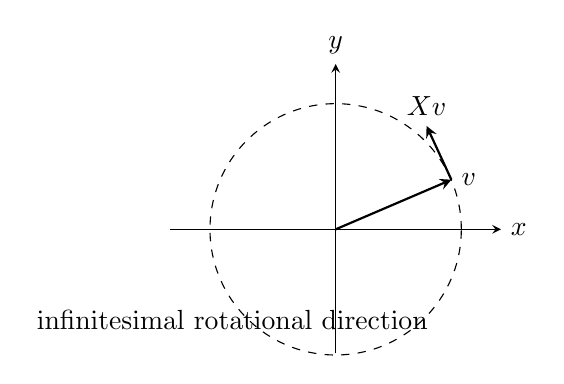
\begin{tikzpicture}[scale=1.05,>=stealth]
\draw[->] (-2,0)--(2,0) node[right]{\(x\)};
\draw[->] (0,-1.5)--(0,2) node[above]{\(y\)};

\draw[thick,->] (0,0)--(1.4,0.6) node[right]{\(v\)};
\draw[thick,->] (1.4,0.6)--(1.1,1.25) node[above]{\(Xv\)};

\draw[dashed] (0,0) circle (1.52);
\node at (-1.25,-1.1) {infinitesimal rotational direction};
\end{tikzpicture}
\end{center}

A Lie algebra element represents an instantaneous direction of motion rather
than a completed finite rotation.

%%%%%%%%%%%%%%%%%%%%%%%%%%%%%%%%%%%%%%%%%%%%%%%%%%%%%%%%%%%%
\subsection{Simple Lie Algebras}
\label{subsec:simple-lie-algebras}
%%%%%%%%%%%%%%%%%%%%%%%%%%%%%%%%%%%%%%%%%%%%%%%%%%%%%%%%%%%%

\begin{definitionbox}{Simple Lie Algebra}
A nonabelian Lie algebra \(\mathfrak g\) is \emph{simple} if its only ideals
are
\[ \{0\}\qquad\text{and}\qquad\mathfrak g. \]
\end{definitionbox}

This resembles the notion of simple groups and simple modules.

Simple Lie algebras form fundamental building blocks in Lie theory.

Over suitable fields, many important Lie algebras such as

\[ \mathfrak{sl}_n \]

are simple, subject to characteristic restrictions and low-dimensional
exceptions.

%%%%%%%%%%%%%%%%%%%%%%%%%%%%%%%%%%%%%%%%%%%%%%%%%%%%%%%%%%%%
\subsection{Solvable Lie Algebras}
\label{subsec:solvable-lie-algebras}
%%%%%%%%%%%%%%%%%%%%%%%%%%%%%%%%%%%%%%%%%%%%%%%%%%%%%%%%%%%%

Define the derived series by

\[ \mathfrak g^{(0)}=\mathfrak g, \]

\[ \mathfrak g^{(1)}=[\mathfrak g,\mathfrak g], \]

and recursively,

\[ \mathfrak g^{(k+1)}
=[\mathfrak g^{(k)},\mathfrak g^{(k)}]. \]

\begin{definitionbox}{Solvable Lie Algebra}
A Lie algebra \(\mathfrak g\) is \emph{solvable} if
\[ \mathfrak g^{(m)}=0 \]
for some integer \(m\geq0\).
\end{definitionbox}

Abelian Lie algebras are automatically solvable.

%%%%%%%%%%%%%%%%%%%%%%%%%%%%%%%%%%%%%%%%%%%%%%%%%%%%%%%%%%%%
\subsection{Nilpotent Lie Algebras}
\label{subsec:nilpotent-lie-algebras}
%%%%%%%%%%%%%%%%%%%%%%%%%%%%%%%%%%%%%%%%%%%%%%%%%%%%%%%%%%%%

Define the lower central series by

\[ \mathfrak g_1=\mathfrak g, \]

\[ \mathfrak g_{k+1}=[\mathfrak g,\mathfrak g_k]. \]

\begin{definitionbox}{Nilpotent Lie Algebra}
A Lie algebra is \emph{nilpotent} if
\[ \mathfrak g_m=0 \]
for some \(m\).
\end{definitionbox}

Every nilpotent Lie algebra is solvable, but the converse is not generally
true.

%%%%%%%%%%%%%%%%%%%%%%%%%%%%%%%%%%%%%%%%%%%%%%%%%%%%%%%%%%%%
\subsection{Structural Hierarchy}
\label{subsec:lie-algebra-hierarchy}
%%%%%%%%%%%%%%%%%%%%%%%%%%%%%%%%%%%%%%%%%%%%%%%%%%%%%%%%%%%%

\begin{center}
\begin{tikzpicture}[
    node distance=12mm,
    box/.style={draw,rounded corners,align=center,inner sep=5pt},
    >=stealth
]
\node[box] (abel) {Abelian};
\node[box,below=of abel] (nil) {Nilpotent};
\node[box,below=of nil] (solv) {Solvable};
\node[box,below=of solv] (general) {General Lie algebra};

\draw[->,thick] (abel)--node[right]{implies}(nil);
\draw[->,thick] (nil)--node[right]{implies}(solv);
\draw[->,thick] (solv)--(general);
\end{tikzpicture}
\end{center}

Simple Lie algebras belong to a different structural direction: they are
nonabelian Lie algebras that cannot be decomposed through nontrivial ideals.

%%%%%%%%%%%%%%%%%%%%%%%%%%%%%%%%%%%%%%%%%%%%%%%%%%%%%%%%%%%%
\subsection{Semisimple Lie Algebras}
\label{subsec:semisimple-lie-algebras}
%%%%%%%%%%%%%%%%%%%%%%%%%%%%%%%%%%%%%%%%%%%%%%%%%%%%%%%%%%%%

A complete treatment of semisimple Lie algebras requires substantial
additional theory.

At an introductory level, one may think of semisimple Lie algebras as Lie
algebras built from simple components without nonzero solvable ideals.

Over characteristic zero, finite-dimensional semisimple Lie algebras
decompose into direct sums of simple Lie algebras.

Schematically,

\[ \mathfrak g\cong
\mathfrak g_1\oplus\cdots\oplus\mathfrak g_r, \]

where the \(\mathfrak g_i\) are simple.

%%%%%%%%%%%%%%%%%%%%%%%%%%%%%%%%%%%%%%%%%%%%%%%%%%%%%%%%%%%%
\subsection{The Killing Form}
\label{subsec:killing-form}
%%%%%%%%%%%%%%%%%%%%%%%%%%%%%%%%%%%%%%%%%%%%%%%%%%%%%%%%%%%%

The adjoint representation produces an important bilinear form.

\begin{definitionbox}{Killing Form}
The \emph{Killing form} of a finite-dimensional Lie algebra
\(\mathfrak g\) is
\[ B(X,Y)=\tr(\operatorname{ad}_X\operatorname{ad}_Y). \]
\end{definitionbox}

The capital letter

\[ B \]

here denotes a bilinear form.

The Killing form provides information about the internal structure of the
Lie algebra.

In characteristic zero, Cartan's criterion states that a finite-dimensional
Lie algebra is semisimple precisely when its Killing form is nondegenerate.

%%%%%%%%%%%%%%%%%%%%%%%%%%%%%%%%%%%%%%%%%%%%%%%%%%%%%%%%%%%%
\subsection{Root-Space Philosophy}
\label{subsec:root-space-philosophy}
%%%%%%%%%%%%%%%%%%%%%%%%%%%%%%%%%%%%%%%%%%%%%%%%%%%%%%%%%%%%

The classification of semisimple Lie algebras relies on decomposing them
relative to suitable commuting subalgebras.

Very roughly, one obtains decompositions of the form

\[ \mathfrak g=\mathfrak h\oplus
\bigoplus_{\alpha\in\Phi}\mathfrak g_\alpha. \]

Here:

\begin{itemize}
    \item \(\mathfrak h\) is a Cartan subalgebra;
    \item \(\Phi\) is a collection of roots;
    \item \(\mathfrak g_\alpha\) are root spaces.
\end{itemize}

The Greek letter

\[ \alpha \]

is alpha, pronounced ``AL-fuh.''

The capital Greek letter

\[ \Phi \]

is Phi, commonly pronounced ``fie'' or ``fee.''

This theory leads to root systems and Dynkin diagrams.

A full classification belongs to advanced Lie theory and is not developed
in detail here.

%%%%%%%%%%%%%%%%%%%%%%%%%%%%%%%%%%%%%%%%%%%%%%%%%%%%%%%%%%%%
\subsection{Dynkin Diagrams: A Preview}
\label{subsec:dynkin-diagrams-preview}
%%%%%%%%%%%%%%%%%%%%%%%%%%%%%%%%%%%%%%%%%%%%%%%%%%%%%%%%%%%%

Dynkin diagrams encode the root systems of semisimple Lie algebras.

Examples include

\begin{center}
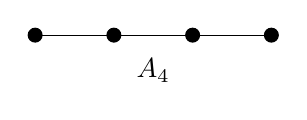
\begin{tikzpicture}[scale=1]
\foreach \x in {0,1,2,3}
    \filldraw (\x,0) circle (2.5pt);
\draw (0,0)--(1,0)--(2,0)--(3,0);
\node at (1.5,-0.45) {\(A_4\)};
\end{tikzpicture}
\qquad\qquad
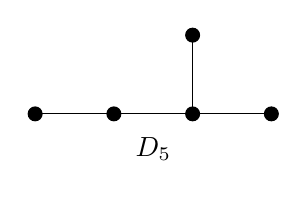
\begin{tikzpicture}[scale=1]
\filldraw (0,0) circle (2.5pt);
\filldraw (1,0) circle (2.5pt);
\filldraw (2,0) circle (2.5pt);
\filldraw (3,0) circle (2.5pt);
\filldraw (2,1) circle (2.5pt);
\draw (0,0)--(1,0)--(2,0)--(3,0);
\draw (2,0)--(2,1);
\node at (1.5,-0.45) {\(D_5\)};
\end{tikzpicture}
\end{center}

The major infinite families are traditionally denoted

\[ A_n,\qquad B_n,\qquad C_n,\qquad D_n, \]

together with exceptional types

\[ E_6,\ E_7,\ E_8,\ F_4,\ G_2. \]

These diagrams are classification tools rather than ordinary graphs arising
from graph theory.

%%%%%%%%%%%%%%%%%%%%%%%%%%%%%%%%%%%%%%%%%%%%%%%%%%%%%%%%%%%%
\subsection{Lie Theory and Representation Theory}
\label{subsec:lie-representation-connection}
%%%%%%%%%%%%%%%%%%%%%%%%%%%%%%%%%%%%%%%%%%%%%%%%%%%%%%%%%%%%

Representation theory becomes especially powerful when applied to Lie groups
and Lie algebras.

A Lie group representation

\[ \rho:G\to GL(V) \]

can often be differentiated to obtain a Lie algebra representation

\[ d\rho:\mathfrak g\to\mathfrak{gl}(V). \]

Thus one may replace a nonlinear group problem with a linearized Lie algebra
problem.

\begin{center}
\begin{tikzcd}[column sep=large,row sep=large]
G \arrow[r,"\rho"] \arrow[d,"\text{differentiate}"'] &
GL(V) \arrow[d,"\text{differentiate}"]\\
\mathfrak g \arrow[r,"d\rho"'] &
\mathfrak{gl}(V)
\end{tikzcd}
\end{center}

%%%%%%%%%%%%%%%%%%%%%%%%%%%%%%%%%%%%%%%%%%%%%%%%%%%%%%%%%%%%
\subsection{Lie Theory and Geometry}
\label{subsec:lie-theory-geometry}
%%%%%%%%%%%%%%%%%%%%%%%%%%%%%%%%%%%%%%%%%%%%%%%%%%%%%%%%%%%%

Lie groups are geometric spaces with symmetry built directly into their
structure.

They appear naturally as:

\begin{itemize}
    \item groups of rotations;
    \item groups of rigid motions;
    \item transformation groups of manifolds;
    \item symmetry groups of geometric structures;
    \item matrix groups preserving bilinear or Hermitian forms.
\end{itemize}

The tangent-space construction

\[ G\longmapsto T_eG=\mathfrak g \]

is one of the fundamental bridges between algebra and differential geometry.

%%%%%%%%%%%%%%%%%%%%%%%%%%%%%%%%%%%%%%%%%%%%%%%%%%%%%%%%%%%%
\subsection{Lie Theory and Physics}
\label{subsec:lie-theory-physics}
%%%%%%%%%%%%%%%%%%%%%%%%%%%%%%%%%%%%%%%%%%%%%%%%%%%%%%%%%%%%

Continuous physical symmetries are naturally described by Lie groups.

Examples include:

\begin{itemize}
    \item \(SO(3)\) for spatial rotations;
    \item \(SU(2)\) in spin and quantum mechanics;
    \item \(U(1)\) in phase symmetry;
    \item \(SU(3)\) in particle physics;
    \item Lorentz and Poincaré groups in relativity.
\end{itemize}

The corresponding Lie algebras describe infinitesimal symmetry generators.

For example, angular momentum operators arise as infinitesimal generators of
rotational symmetry.

%%%%%%%%%%%%%%%%%%%%%%%%%%%%%%%%%%%%%%%%%%%%%%%%%%%%%%%%%%%%
\subsection{Lie Theory and Control}
\label{subsec:lie-theory-control}
%%%%%%%%%%%%%%%%%%%%%%%%%%%%%%%%%%%%%%%%%%%%%%%%%%%%%%%%%%%%

Many mechanical systems evolve on spaces that are themselves Lie groups.

Examples include:

\begin{itemize}
    \item orientation of aircraft and spacecraft;
    \item robot motion;
    \item rigid-body dynamics;
    \item navigation and attitude estimation.
\end{itemize}

Three-dimensional orientation naturally belongs to

\[ SO(3), \]

rather than an ordinary Euclidean vector space.

Rigid motions in three-dimensional space are described by the special
Euclidean group

\[ SE(3). \]

Lie theory therefore provides natural mathematical coordinates for many
control and robotics problems.

%%%%%%%%%%%%%%%%%%%%%%%%%%%%%%%%%%%%%%%%%%%%%%%%%%%%%%%%%%%%
\subsection{The Special Euclidean Group}
\label{subsec:special-euclidean-group}
%%%%%%%%%%%%%%%%%%%%%%%%%%%%%%%%%%%%%%%%%%%%%%%%%%%%%%%%%%%%

Rigid motions combine rotations and translations.

In three dimensions, they can be represented by matrices

\[ 
\begin{pmatrix}
R&p\\
0&1
\end{pmatrix},
\qquad R\in SO(3),\quad p\in\R^3.
\]

These matrices form

\[ SE(3), \]

the \emph{special Euclidean group}.

The notation is read ``special Euclidean group of dimension three.''

Its multiplication combines rotational and translational motion.

%%%%%%%%%%%%%%%%%%%%%%%%%%%%%%%%%%%%%%%%%%%%%%%%%%%%%%%%%%%%
\subsection{A Structural Map of Lie Theory}
\label{subsec:lie-theory-structural-map}
%%%%%%%%%%%%%%%%%%%%%%%%%%%%%%%%%%%%%%%%%%%%%%%%%%%%%%%%%%%%

\begin{center}
\begin{tikzpicture}[
    node distance=11mm and 16mm,
    box/.style={draw,rounded corners,align=center,inner sep=5pt,font=\small},
    >=stealth
]
\node[box] (sym) {Continuous\\symmetry};
\node[box,below=of sym] (group) {Lie group \(G\)};
\node[box,below left=of group] (geo) {Global\\geometry};
\node[box,below right=of group] (alg) {Lie algebra\\\(\mathfrak g=T_eG\)};
\node[box,below=of alg] (bracket) {Lie bracket\\\([X,Y]\)};
\node[box,below left=of bracket] (rep) {Representations};
\node[box,below right=of bracket] (struct) {Structure theory};
\node[box,below=26mm of bracket] (apps) {Geometry, differential equations,\\physics, control, topology};

\draw[->] (sym)--(group);
\draw[->] (group)--(geo);
\draw[->] (group)--node[right]{differentiate}(alg);
\draw[->] (alg)--(bracket);
\draw[->] (bracket)--(rep);
\draw[->] (bracket)--(struct);
\draw[->] (geo)--(apps);
\draw[->] (rep)--(apps);
\draw[->] (struct)--(apps);
\end{tikzpicture}
\end{center}

%%%%%%%%%%%%%%%%%%%%%%%%%%%%%%%%%%%%%%%%%%%%%%%%%%%%%%%%%%%%
\subsection{Worked Example: Checking a Lie Subalgebra}
\label{subsec:worked-lie-subalgebra}
%%%%%%%%%%%%%%%%%%%%%%%%%%%%%%%%%%%%%%%%%%%%%%%%%%%%%%%%%%%%

\begin{workedexamplebox}{Diagonal Matrices as a Lie Subalgebra}

Let \(\mathfrak h\) be the set of diagonal \(2\times2\) real matrices.
Determine whether \(\mathfrak h\) is a Lie subalgebra of
\(\mathfrak{gl}_2(\R)\).

\begin{tabularx}{\textwidth}{@{}>{\raggedright\arraybackslash}p{0.42\textwidth}X@{}}
Choose two elements. &
\(\displaystyle X=\begin{pmatrix}a&0\\0&b\end{pmatrix},\
Y=\begin{pmatrix}c&0\\0&d\end{pmatrix}\)\\
Diagonal matrices commute. & \(XY=YX\)\\
Compute the bracket. & \([X,Y]=XY-YX=0\)\\
Check closure. & \(0\in\mathfrak h\)
\end{tabularx}

\begin{answerbox}
\[ \boxed{\mathfrak h\text{ is an abelian Lie subalgebra of }
\mathfrak{gl}_2(\R).} \]
\end{answerbox}
\end{workedexamplebox}

%%%%%%%%%%%%%%%%%%%%%%%%%%%%%%%%%%%%%%%%%%%%%%%%%%%%%%%%%%%%
\subsection{Worked Example: Center of \(\mathfrak{gl}_n(F)\)}
\label{subsec:worked-center-gln}
%%%%%%%%%%%%%%%%%%%%%%%%%%%%%%%%%%%%%%%%%%%%%%%%%%%%%%%%%%%%

\begin{workedexamplebox}{Scalar Matrices and the Center}

Show that every scalar matrix

\[ X=\lambda I \]

lies in the center of \(\mathfrak{gl}_n(F)\).

\begin{tabularx}{\textwidth}{@{}>{\raggedright\arraybackslash}p{0.42\textwidth}X@{}}
Choose any \(Y\in\mathfrak{gl}_n(F)\). & \(Y\in M_n(F)\)\\
Compute \(XY\). & \(XY=(\lambda I)Y=\lambda Y\)\\
Compute \(YX\). & \(YX=Y(\lambda I)=\lambda Y\)\\
Compute the bracket. & \([X,Y]=XY-YX=0\)
\end{tabularx}

\begin{answerbox}
\[ \boxed{\lambda I\in Z(\mathfrak{gl}_n(F)).} \]
\end{answerbox}
\end{workedexamplebox}

%%%%%%%%%%%%%%%%%%%%%%%%%%%%%%%%%%%%%%%%%%%%%%%%%%%%%%%%%%%%
\subsection{Common Errors}
\label{subsec:lie-theory-common-errors}
%%%%%%%%%%%%%%%%%%%%%%%%%%%%%%%%%%%%%%%%%%%%%%%%%%%%%%%%%%%%

\subsubsection{Treating Every Group as a Lie Group}

A Lie group requires compatible smooth geometric structure.

Finite groups are important groups, but as positive-dimensional continuous
symmetry spaces they behave very differently from groups such as \(SO(n)\)
or \(GL_n(\R)\).

%%%%%%%%%%%%%%%%%%%%%%%%%%%%%%%%%%%%%%%%%%%%%%%%%%%%%%%%%%%%
\subsubsection{Confusing a Lie Group with Its Lie Algebra}

A Lie group \(G\) is generally nonlinear and has a group multiplication.

Its Lie algebra

\[ \mathfrak g=T_eG \]

is a vector space equipped with a Lie bracket.

They are related but are not the same object.

%%%%%%%%%%%%%%%%%%%%%%%%%%%%%%%%%%%%%%%%%%%%%%%%%%%%%%%%%%%%
\subsubsection{Assuming the Lie Bracket Is Ordinary Multiplication}

For matrix Lie algebras,

\[ [X,Y]=XY-YX, \]

not simply \(XY\).

%%%%%%%%%%%%%%%%%%%%%%%%%%%%%%%%%%%%%%%%%%%%%%%%%%%%%%%%%%%%
\subsubsection{Assuming the Lie Bracket Is Associative}

In general,

\[ [X,[Y,Z]]\neq[[X,Y],Z]. \]

The correct structural identity is the Jacobi identity.

%%%%%%%%%%%%%%%%%%%%%%%%%%%%%%%%%%%%%%%%%%%%%%%%%%%%%%%%%%%%
\subsubsection{Assuming Matrix Exponentials Always Add Normally}

The identity

\[ e^{X+Y}=e^Xe^Y \]

generally requires

\[ [X,Y]=0. \]

Noncommuting matrices require commutator corrections.

%%%%%%%%%%%%%%%%%%%%%%%%%%%%%%%%%%%%%%%%%%%%%%%%%%%%%%%%%%%%
\subsubsection{Confusing \(SO(n)\) with \(O(n)\)}

The orthogonal group allows

\[ \det(A)=\pm1. \]

The special orthogonal group requires

\[ \det(A)=1. \]

Thus

\[ SO(n)\subseteq O(n). \]

%%%%%%%%%%%%%%%%%%%%%%%%%%%%%%%%%%%%%%%%%%%%%%%%%%%%%%%%%%%%
\subsubsection{Confusing \(\operatorname{Ad}\) and \(\operatorname{ad}\)}

The capitalized map

\[ \operatorname{Ad} \]

acts at the Lie group level.

The lowercase map

\[ \operatorname{ad} \]

acts at the Lie algebra level.

%%%%%%%%%%%%%%%%%%%%%%%%%%%%%%%%%%%%%%%%%%%%%%%%%%%%%%%%%%%%
\subsubsection{Assuming the Lie Algebra Determines the Entire Group}

The Lie algebra determines local infinitesimal structure but may not
determine global topology.

Different Lie groups can have isomorphic Lie algebras.

%%%%%%%%%%%%%%%%%%%%%%%%%%%%%%%%%%%%%%%%%%%%%%%%%%%%%%%%%%%%
\subsection{Applications}
\label{subsec:lie-theory-applications}
%%%%%%%%%%%%%%%%%%%%%%%%%%%%%%%%%%%%%%%%%%%%%%%%%%%%%%%%%%%%

\begin{applicationbox}
\textbf{Geometry.}
Lie groups describe continuous transformation groups of geometric spaces,
while Lie algebras describe their infinitesimal motions.

\medskip

\textbf{Differential Equations.}
Matrix exponentials and one-parameter subgroups describe flows of linear
systems and symmetry-preserving differential equations.

\medskip

\textbf{Representation Theory.}
Representations of Lie groups can often be differentiated into
representations of Lie algebras, converting nonlinear symmetry into linear
algebra.

\medskip

\textbf{Mathematical Physics.}
Rotations, quantum symmetries, gauge symmetries, and conservation laws are
naturally expressed using Lie groups and Lie algebras.

\medskip

\textbf{Robotics and Aerospace.}
Orientation and rigid-body motion are modeled using groups such as
\(SO(3)\) and \(SE(3)\).

\medskip

\textbf{Control Theory.}
Control systems evolving on nonlinear configuration spaces frequently use
Lie-group geometry and Lie-algebra linearization.

\medskip

\textbf{Topology.}
The global topology of Lie groups interacts deeply with covering spaces,
homotopy, and manifold theory.

\medskip

\textbf{Number Theory and Algebra.}
Algebraic groups and their representations connect Lie-theoretic ideas with
arithmetic, algebraic geometry, and modern representation theory.
\end{applicationbox}

%%%%%%%%%%%%%%%%%%%%%%%%%%%%%%%%%%%%%%%%%%%%%%%%%%%%%%%%%%%%
\subsection{Exercises}
\label{subsec:lie-theory-exercises}
%%%%%%%%%%%%%%%%%%%%%%%%%%%%%%%%%%%%%%%%%%%%%%%%%%%%%%%%%%%%

\begin{exercise}[1]
Explain in words what distinguishes a Lie group from an ordinary abstract
group.
\end{exercise}

\begin{exercise}[1]
Show that \((\R,+)\) is a Lie group.
\end{exercise}

\begin{exercise}[1]
Show that \((\R_{>0},\cdot)\) is a Lie group.
\end{exercise}

\begin{exercise}[2]
Verify that
\[ \exp:(\R,+)\to(\R_{>0},\cdot) \]
is a group isomorphism.
\end{exercise}

\begin{exercise}[1]
Write the general form of an element of \(SO(2)\).
\end{exercise}

\begin{exercise}[2]
Verify directly that
\[ R(\theta)R(\phi)=R(\theta+\phi). \]
\end{exercise}

\begin{exercise}[1]
Define \(GL_n(\R)\).
\end{exercise}

\begin{exercise}[1]
Define \(SL_n(\R)\).
\end{exercise}

\begin{exercise}[1]
Define \(O(n)\) and \(SO(n)\).
\end{exercise}

\begin{exercise}[1]
Define \(U(n)\) and \(SU(n)\).
\end{exercise}

\begin{exercise}[2]
Show that the product of two matrices in \(SL_n(\R)\) remains in
\(SL_n(\R)\).
\end{exercise}

\begin{exercise}[2]
Show that if \(A\in O(n)\), then
\[ A^{-1}=A^{\mathsf T}. \]
\end{exercise}

\begin{exercise}[1]
State the definition of a Lie algebra.
\end{exercise}

\begin{exercise}[1]
State the Jacobi identity.
\end{exercise}

\begin{exercise}[1]
Define the matrix commutator.
\end{exercise}

\begin{exercise}[2]
Show that
\[ [X,Y]=-[Y,X]. \]
\end{exercise}

\begin{exercise}[2]
Show that
\[ [X,X]=0. \]
\end{exercise}

\begin{exercise}[2]
Verify bilinearity of the matrix commutator.
\end{exercise}

\begin{exercise}[3]
Expand the matrix commutators and verify the Jacobi identity directly.
\end{exercise}

\begin{exercise}[1]
Define \(\mathfrak{gl}_n(F)\).
\end{exercise}

\begin{exercise}[1]
Determine
\[ \dim\mathfrak{gl}_4(F). \]
\end{exercise}

\begin{exercise}[2]
Prove
\[ [E_{ij},E_{kl}]
=\delta_{jk}E_{il}-\delta_{li}E_{kj}. \]
\end{exercise}

\begin{exercise}[1]
Define \(\mathfrak{sl}_n(F)\).
\end{exercise}

\begin{exercise}[2]
Show that the commutator of two traceless matrices is traceless.
\end{exercise}

\begin{exercise}[1]
Determine
\[ \dim\mathfrak{sl}_5(F). \]
\end{exercise}

\begin{exercise}[2]
Verify the relations
\[ [H,E]=2E,\qquad[H,F]=-2F,\qquad[E,F]=H \]
for the standard basis of \(\mathfrak{sl}_2(F)\).
\end{exercise}

\begin{exercise}[1]
Define \(\mathfrak{so}(n)\).
\end{exercise}

\begin{exercise}[2]
Prove
\[ \dim\mathfrak{so}(n)=\frac{n(n-1)}{2}. \]
\end{exercise}

\begin{exercise}[1]
Describe every element of \(\mathfrak{so}(2)\).
\end{exercise}

\begin{exercise}[2]
Show that the commutator of two skew-symmetric matrices is skew-symmetric.
\end{exercise}

\begin{exercise}[1]
Define \(\mathfrak{u}(n)\).
\end{exercise}

\begin{exercise}[2]
Show that the commutator of two skew-Hermitian matrices is skew-Hermitian.
\end{exercise}

\begin{exercise}[1]
Define a one-parameter subgroup.
\end{exercise}

\begin{exercise}[2]
Show that
\[ \gamma(t)=e^{tX} \]
is a one-parameter subgroup whenever \(X\) is a fixed matrix.
\end{exercise}

\begin{exercise}[1]
Write the power-series definition of \(e^X\).
\end{exercise}

\begin{exercise}[2]
Let
\[ X=\begin{pmatrix}a&0\\0&b\end{pmatrix}. \]
Compute \(e^X\).
\end{exercise}

\begin{exercise}[2]
Let
\[ N=\begin{pmatrix}0&1\\0&0\end{pmatrix}. \]
Compute \(e^{tN}\).
\end{exercise}

\begin{exercise}[2]
Using \(J^2=-I\), derive
\[ e^{\theta J}=I\cos\theta+J\sin\theta. \]
\end{exercise}

\begin{exercise}[2]
Give an example of matrices \(X,Y\) for which
\[ e^{X+Y}\neq e^Xe^Y. \]
\end{exercise}

\begin{exercise}[1]
Define a Lie subalgebra.
\end{exercise}

\begin{exercise}[1]
Define an ideal of a Lie algebra.
\end{exercise}

\begin{exercise}[2]
Prove that the center \(Z(\mathfrak g)\) is an ideal.
\end{exercise}

\begin{exercise}[2]
Prove that
\[ [\mathfrak g,\mathfrak g] \]
is an ideal of \(\mathfrak g\).
\end{exercise}

\begin{exercise}[1]
Define a Lie algebra homomorphism.
\end{exercise}

\begin{exercise}[2]
Show that the kernel of a Lie algebra homomorphism is an ideal.
\end{exercise}

\begin{exercise}[2]
Show that the image of a Lie algebra homomorphism is a Lie subalgebra.
\end{exercise}

\begin{exercise}[2]
Prove the First Isomorphism Theorem for Lie algebras.
\end{exercise}

\begin{exercise}[1]
Define structure constants.
\end{exercise}

\begin{exercise}[2]
Find the structure constants of \(\mathfrak{sl}_2(F)\) relative to the basis
\[ E,F,H. \]
\end{exercise}

\begin{exercise}[1]
Define a representation of a Lie algebra.
\end{exercise}

\begin{exercise}[1]
Define the adjoint map
\[ \operatorname{ad}_X. \]
\end{exercise}

\begin{exercise}[2]
Use the Jacobi identity to prove
\[ \operatorname{ad}_{[X,Y]}
=[\operatorname{ad}_X,\operatorname{ad}_Y]. \]
\end{exercise}

\begin{exercise}[2]
Prove
\[ \Ker(\operatorname{ad})=Z(\mathfrak g). \]
\end{exercise}

\begin{exercise}[1]
Explain the difference between
\[ \operatorname{Ad} \]
and
\[ \operatorname{ad}. \]
\end{exercise}

\begin{exercise}[2]
Differentiate
\[ A(t)^{\mathsf T}A(t)=I \]
at \(t=0\) to derive the defining condition for \(\mathfrak{so}(n)\).
\end{exercise}

\begin{exercise}[2]
Use
\[ \det(I+tX)=1+t\tr(X)+O(t^2) \]
to explain why the Lie algebra of \(SL_n(\R)\) consists of traceless
matrices.
\end{exercise}

\begin{exercise}[2]
Show that the diagonal matrices form an abelian Lie subalgebra of
\(\mathfrak{gl}_n(F)\).
\end{exercise}

\begin{exercise}[2]
Show that the scalar matrices lie in
\[ Z(\mathfrak{gl}_n(F)). \]
\end{exercise}

\begin{exercise}[3]
Show that, over a field where the standard argument applies, the center of
\(\mathfrak{gl}_n(F)\) consists precisely of scalar matrices.
\end{exercise}

\begin{exercise}[1]
Define a solvable Lie algebra.
\end{exercise}

\begin{exercise}[1]
Define a nilpotent Lie algebra.
\end{exercise}

\begin{exercise}[2]
Show that every abelian Lie algebra is nilpotent.
\end{exercise}

\begin{exercise}[2]
Show that every nilpotent Lie algebra is solvable.
\end{exercise}

\begin{exercise}[1]
Define a simple Lie algebra.
\end{exercise}

\begin{exercise}[1]
Define the Killing form.
\end{exercise}

\begin{exercise}[2]
Explain why the Lie algebra of \((\R^n,+)\) is abelian.
\end{exercise}

\begin{exercise}[2]
Describe conceptually why a Lie algebra captures local rather than global
information about a Lie group.
\end{exercise}

\begin{exercise}[2]
Explain how matrix exponentials connect Lie algebras with systems of linear
differential equations.
\end{exercise}

%%%%%%%%%%%%%%%%%%%%%%%%%%%%%%%%%%%%%%%%%%%%%%%%%%%%%%%%%%%%
\subsection{Section Connections}
\label{subsec:lie-theory-connections}
%%%%%%%%%%%%%%%%%%%%%%%%%%%%%%%%%%%%%%%%%%%%%%%%%%%%%%%%%%%%

\chapterconnection{
Lie theory extends the study of symmetry from discrete groups to continuous
transformation groups. A Lie group combines group operations with smooth
geometry, while its tangent space at the identity becomes a Lie algebra that
encodes infinitesimal symmetry through the Lie bracket. Matrix Lie groups
such as \(GL_n\), \(SL_n\), \(SO(n)\), and \(U(n)\) lead naturally to the
classical Lie algebras \(\mathfrak{gl}_n\), \(\mathfrak{sl}_n\),
\(\mathfrak{so}_n\), and \(\mathfrak{u}_n\). The exponential map connects
infinitesimal generators with one-parameter subgroups, while the adjoint
representation connects Lie theory directly with representation theory.
Ideals, quotient Lie algebras, simple and solvable structures, and the
Killing form introduce the structural theory that eventually leads to root
systems and Dynkin diagrams. These ideas connect algebra with differential
geometry, topology, differential equations, control theory, robotics,
quantum mechanics, and mathematical physics.
}

%%%%%%%%%%%%%%%%%%%%%%%%%%%%%%%%%%%%%%%%%%%%%%%%%%%%%%%%%%%%
% SECTION SOURCE TRACKING
%%%%%%%%%%%%%%%%%%%%%%%%%%%%%%%%%%%%%%%%%%%%%%%%%%%%%%%%%%%%

%------------------------------------------------------------
% 1.12 Lie Groups and Lie Algebras
%------------------------------------------------------------
%
% Sources:
%   - Brian C. Hall,
%     Lie Groups, Lie Algebras, and Representations:
%     An Elementary Introduction.
%     Key: hall2015lie
%
% Used for:
%   - introductory Lie group and Lie algebra framework;
%   - matrix Lie groups and their Lie algebras;
%   - matrix commutators and classical examples;
%   - one-parameter subgroups and matrix exponentials;
%   - the exponential map;
%   - adjoint representations;
%   - introductory structural theory;
%   - representation-theoretic connections.
%
% Notes:
%   - Group theory is treated canonically in Section 1.4.
%   - Representation theory is treated canonically in Section 1.11.
%   - Smooth manifold theory and tangent-space geometry receive their
%     canonical treatments in the Geometry and Topology branches.
%   - Differential-equation applications are introduced only as connections;
%     their canonical treatment belongs to Chapter 9.
%   - Root systems, Cartan subalgebras, and Dynkin diagrams are introduced
%     only as previews of advanced Lie theory rather than developed fully.
%   - Physical and control-theoretic examples illustrate the role of
%     continuous symmetry without replacing their later canonical treatments.
%   - Visualizations and pedagogical organization are independently
%     developed for this text.
%
\nocite{hall2015lie}